\section{Results}
This part of the chapter provides the results of the experiment related to the two established hypotheses as well as insights gained from demographical information. Like with Experiment 1, data visualisation is provided by SPSS due to the large data file sizes. A significance level of 0.05 was used for all statistical tests. For the sake of disclosure for any graphs that make use of participant ID's, the author's ID is 5. 

\subsection{Relative Effectiveness}
The first of the null hypotheses to be tested is effectiveness in terms of relative effectiveness. 

\subsubsection{Minimum Time Needed to Defeat Distractors}
As mentioned in Section~\ref{sec:ex2postprocessing}, in order to find a reasonable time period to discard unintentional resets in, it is first necessary to look at the minimum time needed to defeat any distractor. This can be seen in Figure~\ref{fig:minDistractorDefeatTime} where the minimum time is \textasciitilde18.23 seconds.

\begin{figure}[tbph]
    \centering
    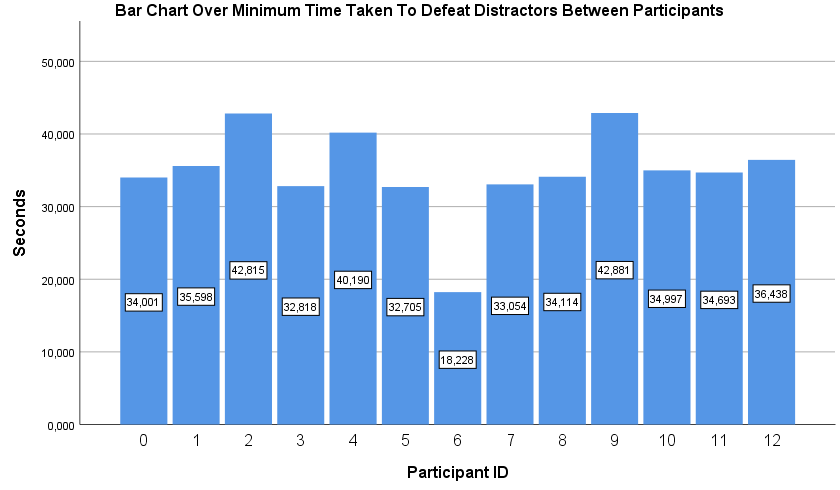
\includegraphics[width=0.75\textwidth]{figures/graphs/MinDistractorDefeatTime.png}
    \caption[Minimum Time Needed To Defeat Distractors Between Participants]{This bar chart shows the minimum time needed for each participant do defeat any distractor in Ensemble Retriever.}
    \label{fig:minDistractorDefeatTime}
\end{figure}

\subsubsection{Time and Walking Speed Normalisation}
Two variables that potentially could have some effect on the the reset counts between conditions is the time spent on walking and the walking speed of participants. It is thus necessary to first look at the mean movement speed and mean time spent on walking between the conditions before further analysis can take place. A boxplot on the time spent walking for participants between the two conditions can be seen in Figure~\ref{fig:TimeSpentWalkingBetweenConditions}. A boxplot on the mean metres per second that participants walked at between conditions can be seen in Figure~\ref{fig:ex2mps}.

\begin{figure}[tbph]
    \centering
    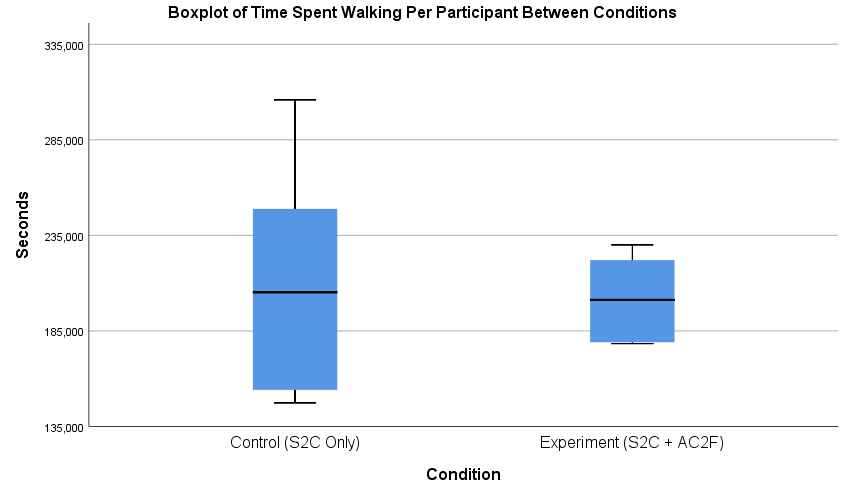
\includegraphics[width=0.75\textwidth]{figures/graphs/TimeSpentWalkingBetweenConditionsBoxPlot.png}
    \caption[Boxplot of Time Spent Walking Between Conditions in Experiment 2]{This boxplot shows the time that participants spent on walking between the two conditions.}
    \label{fig:TimeSpentWalkingBetweenConditions}
\end{figure}

\begin{figure}[tbph]
    \centering
    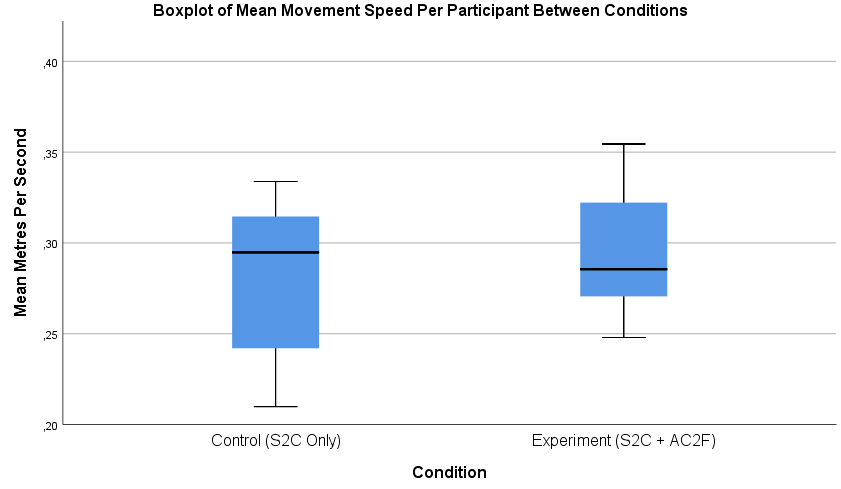
\includegraphics[width=0.75\textwidth]{figures/graphs/mpsBoxplot.png}
    \caption[Boxplot of Mean Walking Speed Between Conditions in Experiment 2]{This boxplot shows the mean walking speeds of participants between conditions.}
    \label{fig:ex2mps}
\end{figure}

A Shapiro-Wilk test was employed to check the normal distribution of these two variables. For the time spent walking, the test provided $p = 0.195$ for S2C Only and $p = 0.490$ for S2C+AC2F. Both conditions are as such normally distributed and a independent samples t-test was employed to look for statistically significant differences. The independent samples t-test yielded $t = 0.262, p = 0.798$ which means there is no statistical significance in terms of time spent walking. For clarity's sake, the mean walking time for S2C Only was 209.2 seconds and 202.0 seconds for S2C+AC2F. 

In terms of the mean walking speed, the Shapiro-Wilk test provided $p = 0.472$ for S2C Only and $p = 0.847$ for S2C+AC2F, meaning that the data is normally distributed. As such, an independent samples t-test was employed to look for statistically significant differences. The independent samples t-test provided $t = -0.633, p = 0.540$ showing that there is no statistically significant difference for walking speeds either. For clarity's sake, the mean walking speed for S2C Only was 0.278 metres per second and 0.294 metres per second for S2C+AC2F.

Since there is no statistically significant difference between the two conditions in terms of time spent walking or walking speed, further analysis will focus on the mean number of legitimate resets per participant. If there would have been a significant difference, a time or speed normalised variable would have needed to be calculated for comparisons. 

\subsubsection{Number of Resets for Participants Between Conditions}
The mean number of resets that participants experienced between conditions can be seen in Figure~\ref{fig:ex2resetMeans}. To supplement the means, a boxplot of the same data can be seen in Figure~\ref{fig:ex2resetboxplot}. As a reminder, the data sample used for these graphs consists of legitimate resets only. Unintentional resets have been removed using the data post processing step as mentioned in Section~\ref{sec:ex2postprocessing}.

\begin{figure}[tbph]
    \centering
    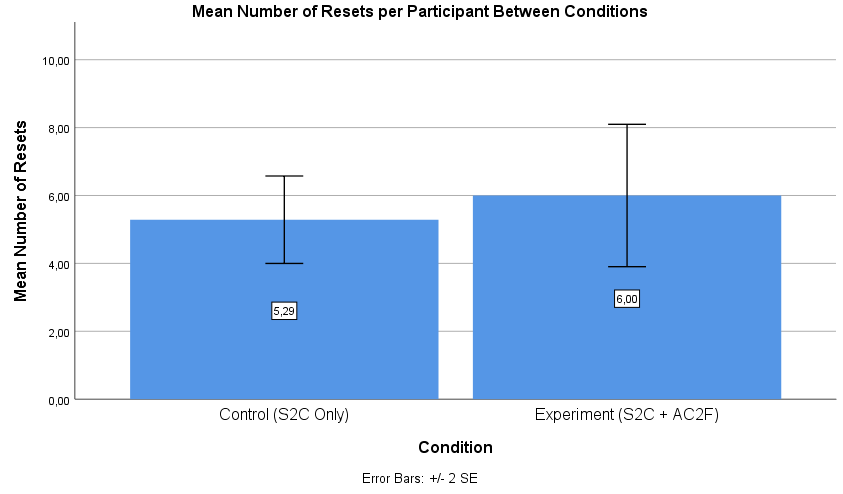
\includegraphics[width=0.75\textwidth]{figures/graphs/ResetMeans.png}
    \caption[Mean Number of Resets Between Conditions for Experiment 2]{This bar chart shows the mean number of resets that participants experienced between conditions.}
    \label{fig:ex2resetMeans}
\end{figure}

\begin{figure}[tbph]
    \centering
    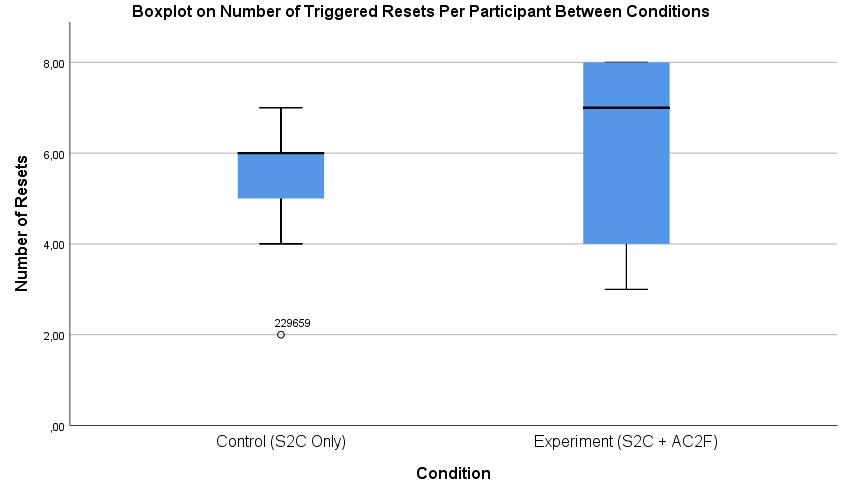
\includegraphics[width=0.75\textwidth]{figures/graphs/resetCountBoxPlot.png}
    \caption[Boxplot on Number of Resets Per Participant Between Conditions for Experiment 2]{This boxplot shows the spread of resets counts that participants experienced between conditions.}
    \label{fig:ex2resetboxplot}
\end{figure}

\subsubsection{Hypothesis Testing}
Finally, in order to test $H_{0_1}$ it is first necessary to test the normality of the data. Using a Shapiro-Wilk test, the S2C Only condition yielded $p = 0.036$ while S2C+AC2F yielded $p = 0.096$. As such, the S2C Only condition is not normally distributed and a non-parametric significance test is needed. In this case, the Mann-Whitney U non-parametric significance test is used. 

Looking at the boxplot in Figure~\ref{fig:ex2resetboxplot}, the overall shape of the distribution is fairly different between the two conditions. As such, the comparison in this case will be on mean ranks only. The Mann-Whitney U test results in $U = 12.500, p = 0.234$. As such, there is no statistically significant difference in terms of number of resets between the two conditions and $H_{0_1}$ is supported.

Since there is no significant difference, the relative effectiveness between the two conditions has not been calculated.

\subsection{Alignment Time Effectiveness}
The second null hypothesis to test is related to effectiveness in terms of time needed to align the user's future path towards the centre of the physical space. 

\subsubsection{Alignment Failure Rates}
Before looking at the processed data sample, it is first necessary to understand the differences in alignment failure rates between the two conditions. Participants in the S2C Only condition triggered 92 distractors in which 22 failed alignment. This results in a failure rate of $23.9\%$. Participants in the S2C+AC2F condition triggered 74 distractors in total and consisted of 6 failed alignments. This results in a failure rate of $8.1\%$. The time taken to defeat the distractor during these failed cases can be seen in Figure~\ref{fig:ex2failedDistractorTimeBoxplot} while the level of the participants' conducting baton during the failure can be seen in Figure~\ref{fig:ex2failedAlignmentBatonLevel}. As seen in Figure~\ref{fig:ex2failedAlignmentBatonLevel}, the S2C Only condition did fail in some cases where the participants' baton was at a lower level, meaning that some failures happened during longer battles. The S2C+AC2F condition on the other hand only failed when the participants' baton was at the maximum level, meaning the alignments failed during the shortest battles. 

\begin{figure}[tbph]
    \centering
    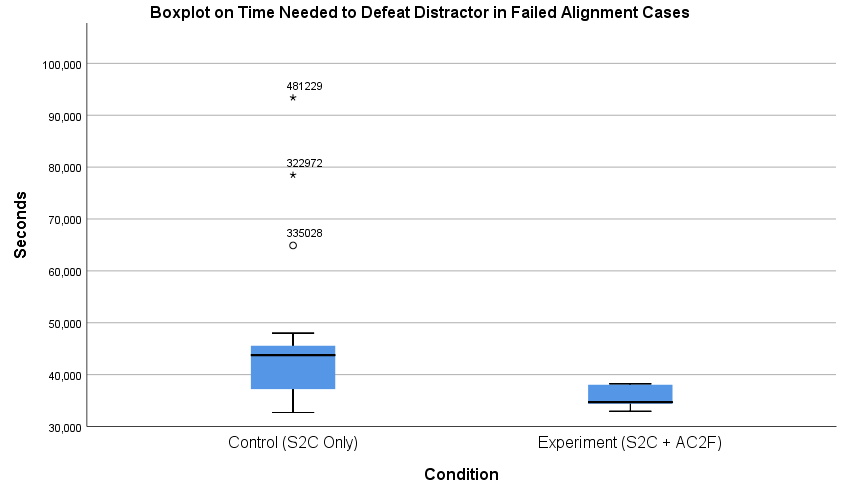
\includegraphics[width=0.75\textwidth]{figures/graphs/failureDistractorDefeatTimeBoxplot.png}
    \caption[Boxplot on Time Needed to Defeat Distractor During Failed Alignments]{This boxplot shows the spread of time in seconds needed to defeat a distractor during the times where alignment towards the centre of the room failed.}
    \label{fig:ex2failedDistractorTimeBoxplot}
\end{figure}

\begin{figure}[tbph]
    \centering
    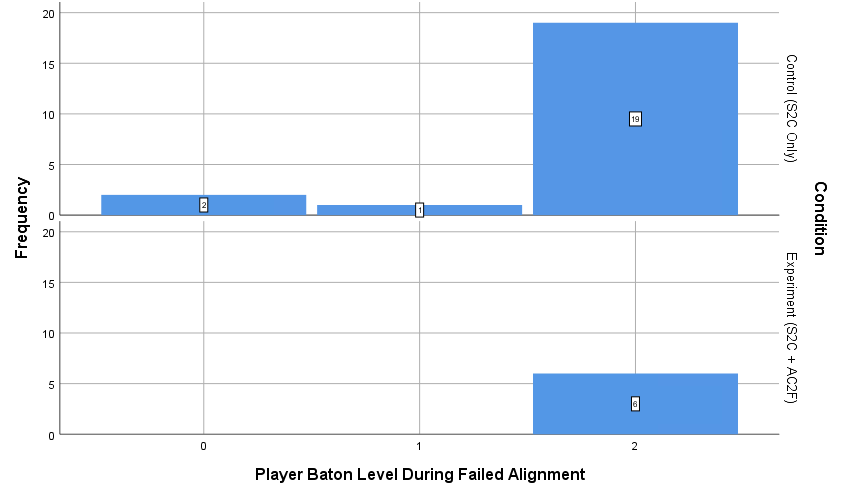
\includegraphics[width=0.75\textwidth]{figures/graphs/failureBatonLevelHistogram.png}
    \caption[Histogram on Player Baton Level During Failed Alignments]{This histogram shows the frequencies of which level the participants' baton was at during failed alignment. Higher levels allows the player to deal more damage.}
    \label{fig:ex2failedAlignmentBatonLevel}
\end{figure}

\subsection{Time Needed for Alignment Between Conditions}
\begin{figure}[tbph]
    \centering
    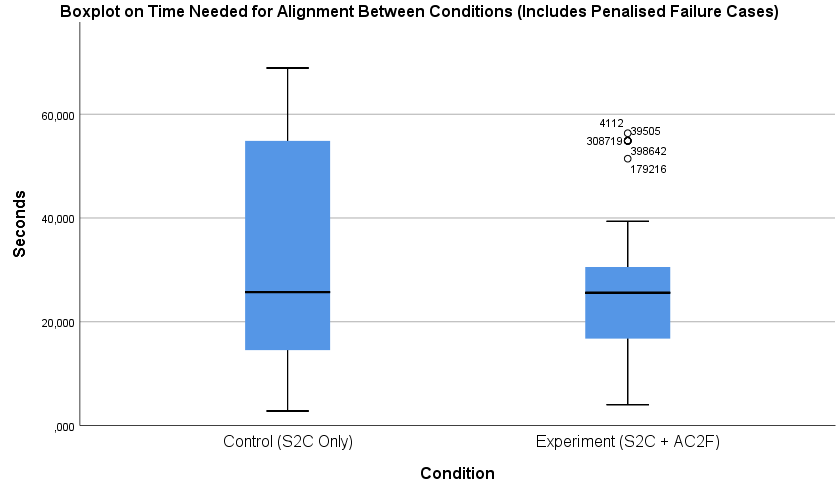
\includegraphics[width=0.75\textwidth]{figures/graphs/boxplotAlignmentTimesWithPenalties.png}
    \caption[Boxplot on Time Needed To Align Participants To Centre (Including Failure Penalties)]{This boxplot shows the spread of time needed to align participants towards the centre of the room. It includes the penalties that are given to cases of failed alignments.}
    \label{fig:alignmentTimesWithPenalties}
\end{figure}

\begin{figure}[tbph]
    \centering
    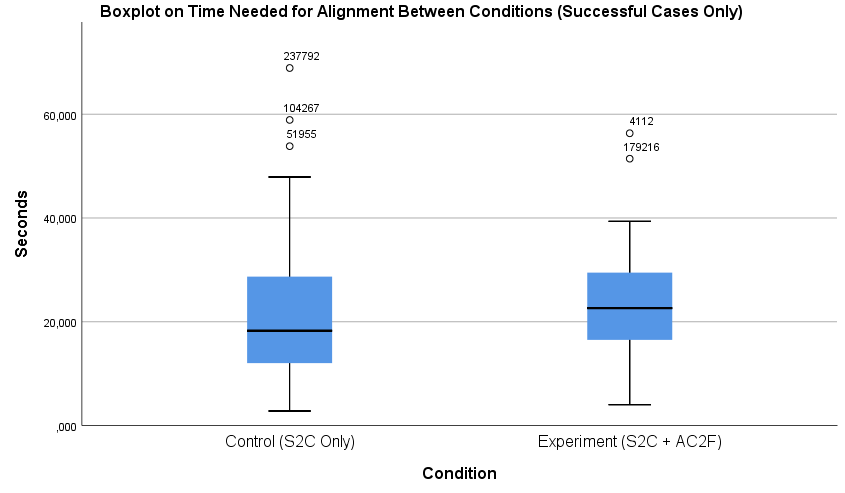
\includegraphics[width=0.75\textwidth]{figures/graphs/boxplotAlignmentTimesWithoutPenalties.png}
    \caption[Boxplot on Time Needed To Align Participants To Centre (Successful Cases Only)]{This boxplot shows the spread of time needed to align participants towards the centre of the room. In this case the data consists of only successful alignments.}
    \label{fig:AlignmentTimesWithoutPenalties}
\end{figure}

Finally, the boxplot showcasing the spread of alignment times with failure penalties can be seen in Figure~\ref{fig:alignmentTimesWithPenalties}. The mean time taken to align the user towards the centre in this case is 30.91 seconds for S2C Only and 25.34 seconds for S2C+AC2F. As a supplement, the spread of alignment times for only successful cases can be seen in Figure~\ref{fig:AlignmentTimesWithoutPenalties}. If failure penalties are disregarded, the mean time needed for alignment is 22.55 seconds for S2C Only and 22.85 for S2C+AC2F. 

\subsubsection{Hypothesis Testing}
In order to test $H_{0_2}$, the data sample including failure penalties will be used. A Shapiro-Wilk normality test was first conducted on the alignment time data. This provided $p < 0.001$ for both conditions and as such, neither is normally distributed. As such, the non-parametric Mann-Whitney U test is used for significance testing. The comparison is done with mean ranks as the shapes in Figure~\ref{fig:alignmentTimesWithPenalties} are fairly different. This results in $U = 2948.500, p = 0.276$, meaning that the test cannot find any statistically significant difference in alignment times. This means that the $H_{0_2}$ null hypothesis is supported. Despite this, it should be noted that the alignment fail rates for the two conditions are different and that the S2C+AC2F condition consisted of $15.8\%$ more successful alignments compared to S2C Only. 

\subsection{Demographical Insights}
Two correlation matrices have been generated from the demographical data in relation to the primary data that is relevant for the hypotheses that have been tested. The Spearman's Rho correlation test has been used to generate the correlation matrices as some of the data is not normally distributed. These correlation matrices can be seen in Figure~\ref{fig:ex2correlation1} and \ref{fig:ex2correlation2}. The correlation test is split into two matrices primarily due to differences in data structure between some of the variables. 

\begin{sidewaysfigure}[tbph]
    \centering
    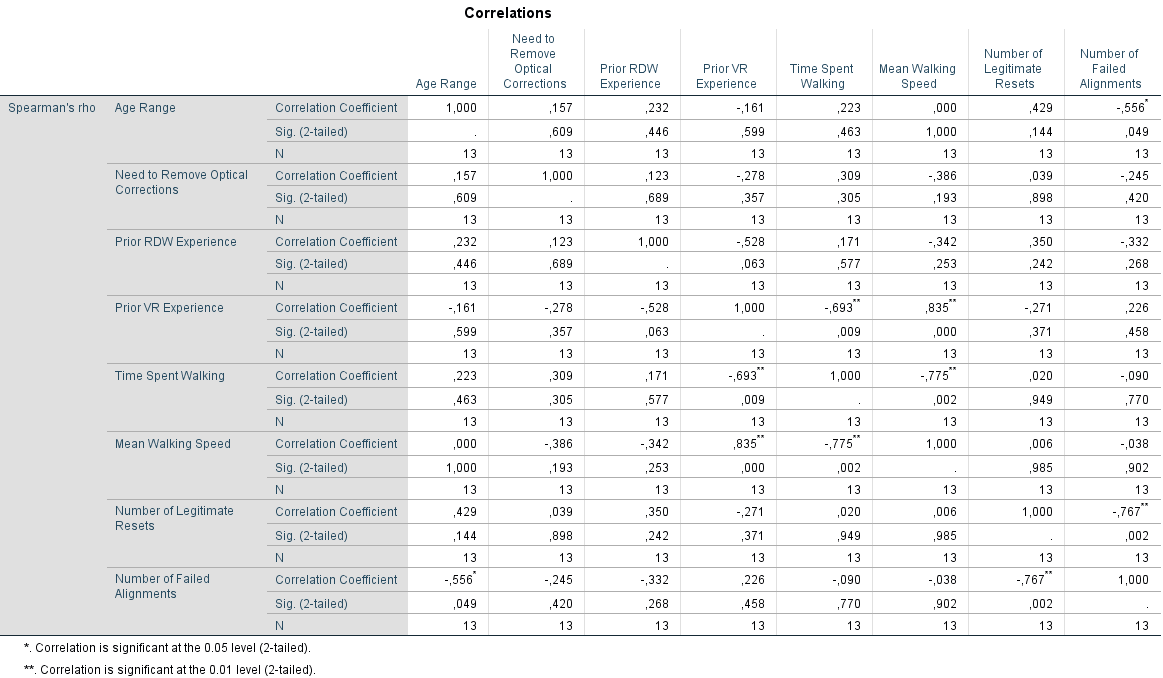
\includegraphics[width=0.9\textwidth]{figures/graphs/Ex2Correlations1.png}
    \caption[Demographical Correlation Matrix 1 for Experiment 2]{Correlation matrix between various demographical variables and relevant variables in Experiment 2.}
    \label{fig:ex2correlation1}
\end{sidewaysfigure}

\begin{figure}[tbph]
    \centering
    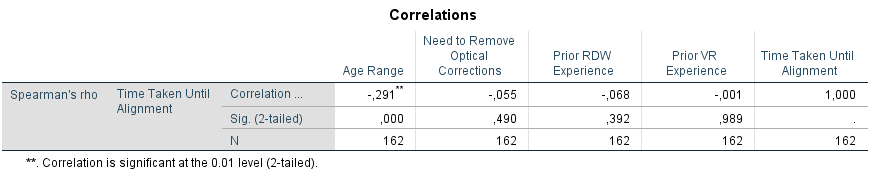
\includegraphics[width=0.9\textwidth]{figures/graphs/Ex2Correlations2.png}
    \caption[Demographical Correlation Matrix 2 for Experiment 2]{Correlation matrix between the time needed to align participants to the centre of the physical space and various demographical variables in Experiment 2.}
    \label{fig:ex2correlation2}
\end{figure}

\subsubsection{Qualitative Feedback}
In terms of qualitative feedback, this section provides a summary of the feedback that participants provided in the questionnaire. The summary is structured after the questions that did receive answers.

\paragraph{Whether the Participants Found Any Bugs or Glitches}
In general, some participants noted that they experienced loss of controller tracking at times. Other than that, no major bugs were experienced by participants.

\paragraph{Whether the Participants Found the Experience Enjoyable}
In general, the participants found the experience to be very enjoyable, although one noted that it was too long for their liking. 

\paragraph{How the Participants Felt About the Redirection Techniques}
Some participants did not notice any redirection, while others did notice it at certain times. The general feedback from participants that did notice the redirection at times was that it felt natural as it was not too strong. In terms of when participants noticed the redirection, it varied a bit. Some had an easier time noticing it in battle, while others found it more easy to notice while walking. The distribution of participants mentioning they noticed the redirection was equal between the two conditions (3 in S2C Only and 3 in S2C+AC2F). 

\paragraph{Whether the Participants Had Any Problems Throughout Their Experience}
The main feedback that was provided for this question was that the physical cable that the HTC Vive uses was rather frustrating to deal with. There were times where participants felt like they had gotten tangled up in the cable and needed to spent some time untangling themselves, somewhat breaking the immersion of the experience. Participants mentioned that the experience would have been substantially improved if integrated with wireless HMD's in the future. 

\subsection{Summary}
The following paragraphs will summarise the results that have been presented in relation to their relevant hypotheses.  

\subsubsection{$H_{0_1}$}
There was no statistically significant difference between the two conditions in terms of mean number of resets per participant (Mann-Whitney U: $U = 12.500, p = 0.234$). As such, no relative effectiveness was calculated and the $H_{0_1}$ null hypothesis is supported.

\subsubsection{$H_{0_2}$}
There was no statistically significant difference between the two conditions in terms of mean time taken to align participants to the centre of the room (Mann-Whitney U: $U = 2948.500, p = 0.276$). Despite this, it should be noted that the alignment failure rates between the two conditions were different. Using S2C together with the AC2F algorithm resulted in $15.8\%$ less alignment failures compared to using only S2C. While the $H_{0_2}$ null hypothesis is supported, the difference in alignment failure rates should be considered.